\documentclass[11pt,a4paper]{article}

\usepackage[english]{babel}
\usepackage[T1]{fontenc}
\usepackage[utf8]{inputenc}
\usepackage{graphicx}
\graphicspath{{../Figs/}}
\usepackage{float}
\usepackage{subcaption}
\usepackage[font=footnotesize,labelfont={sf,bf},textfont=sf,width=\textwidth]{caption}
\usepackage[margin=2cm]{geometry}
\usepackage[plainpages=false,pdfpagelabels,hypertexnames=false]{hyperref}
\usepackage[usenames,dvipsnames]{xcolor}
\usepackage{mathtools}
\usepackage[separate-uncertainty=true]{siunitx}
\usepackage{booktabs}


\title{\bfseries\textsc{Atomic Force Microscopy}}
\author{
Michele Masini\\ \small\texttt{\href{mailto:michele.masini@uni-ulm.de}{michele.masini@uni-ulm.de}}\and
Iyán Méndez Veiga\\ \small\texttt{\href{mailto:iyan.mendez-veiga@uni-ulm.de}{iyan.mendez-veiga@uni-ulm.de}}
}
\date{\today}


\begin{document}
\maketitle

\begin{abstract}
A compact Atomic Force Microscopy (AFM) from Nanosurf company (\href{https://www.nanosurf.com/en/products/naioafm-the-leading-compact-afm}{NaioAFM}) was used to perform measurements of the surface of three samples. Two different operation modes were used: static and tapping mode. Open source software \href{http://gwyddion.net/}{Gwyddion} was used to process the raw data.
\end{abstract}

\vspace{1.5cm}

\section{Introduction}

Since it was first developed in 1985 by \emph{Binning} et al., the Atomic Force Microscopy (AFM) \cite{Bhushan} has become a popular surface profiler for topographic and normal force measurements on the micro- to nanoscale. Not only AFMs, but also modified devices such as Lateral Force Microscopies (LFMs) or Friction Force Microscopies (FFMs), have found applications in different fields.

In this report, we will first describe the AFM technique, the two different operation modes that we tried (static and tapping or dynamic mode) and comment the issues we faced. And secondly, we will describe the processing of raw data obtained from the device using the open source software Gwyddion, as well as a general overview of AFM image artifacts, i.e., features which appear in the images that are not present in the original probed object.

\section{Materials and methods}

\subsection{AFM}

AFM relies on the same idea of Scanning Tunneling Microscope (STM), i.e., using a scanning technique to produce very high resolution, 3D images of sample surfaces. The difference is that instead of measuring tunneling currents, in AFM we measure ultrasmall forces between the tip surface and the sample surface to get the proximity of the tip to the sample, i.e., the height. This allows AFM to measure both conductors and insulators surfaces on an atomic scale.

By ultrasmall forces we mean forces of less than \SI{1}{\nano\N}. How this forces are measured is one of the key aspects of AFM because finding a relation between them and the distance between the tip and the surface will allow us to get a profile of the measured samples. However, this depends on the operation mode.

\begin{figure}[ht]
\centering
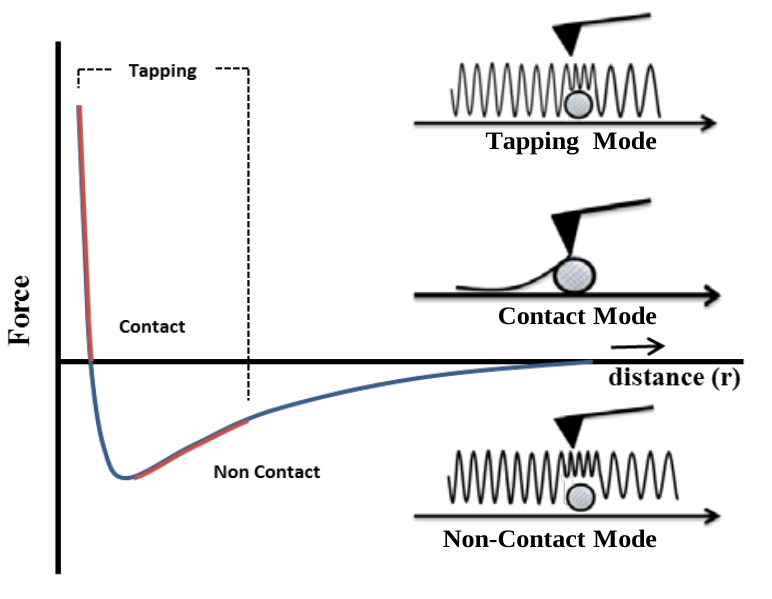
\includegraphics[width=0.7\textwidth]{AFM_modes}
\caption{Force that the tip experiments against the distance with respect to the surface of the sample \cite{jfb8010007}. In the contact mode forces are repulsive while in the non conntact mode are attractive. In the dynamic or tapping mode we are in between but typically closer to the repulsive barrier.}
\label{fig:AFM_modes}
\end{figure}

{\color{red}Basically, we can say that AFM can be used in three modes or regimes} (see Figure \ref{fig:AFM_modes}): static, repulsive or contact mode; dynamic or tapping mode; and non-contact mode. In this report we will talk about the first two.

In the static mode, a sharp tip is brought into contact with the surface of the sample. The tip is placed at the end of a flexible (only in the normal direction) cantilever, which can deflect depending on the force that the tip ``feels''. The repulsive forces are due to electronic orbital overlap between the atoms of the tip and those in the surface of the sample. By measuring the deflection of the cantilever using tunneling, capacitive or optical detectors (see Figure \ref{fig:Deflection_measurement}), we can get a measure of the force if the cantilever spring constant is known.

\begin{figure}[ht]
\centering
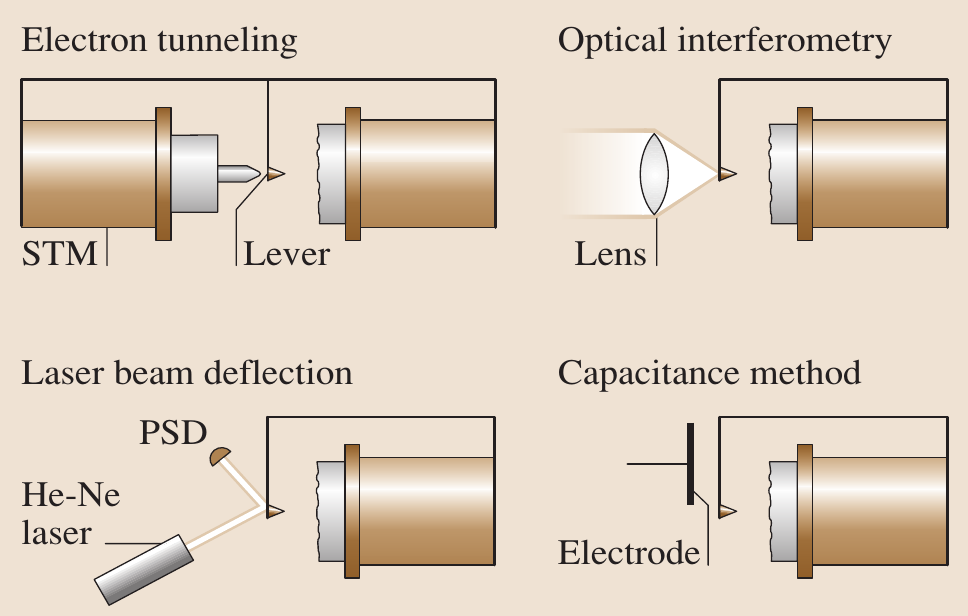
\includegraphics[width=0.5\textwidth]{Deflection}
\caption{Different techniques to measure cantilever deflection in an AFM \cite{Bhushan}.}
\label{fig:Deflection_measurement}
\end{figure}

The deflection can be measured to within \SI{0.02}{\nm}, so for a typical cantilever spring constant of \SI{10}{\N/\m}, forces as low as \SI{0.2}{\nano\N} can be measured.

Typically, the deflection of the cantilever is used as the signal for a feedback mechanism, so whenever due to the profile of the surface there is a change in this deflection, the distance $r$ between the tip and the surface of the sample is modified accordingly using a piezo material. The force that causes this aimed deflection is called \emph{setpoint} and we will see later that it is a key parameter when measuring in this mode. In order to get the profile of the whole surface, either the tip or the sample has to be translated using a piezoelectric scanner.

When we are on the right of the equilibrium (see Figure \ref{fig:AFM_modes}), the attractive forces on the tip are very weak van der Waals forces. Tapping mode can work on this regime but we do not measure the force anymore, but the force gradient. The cantilever is deliberately vibrated in either amplitude modulation (AM) or frequency modulation (FM) at its resonant frequency $\omega_0$ given by the spring constant and the force derivative is determined by measuring the shift in this resonant frequency due to the interaction with the sample.

\begin{figure}[ht]
\centering
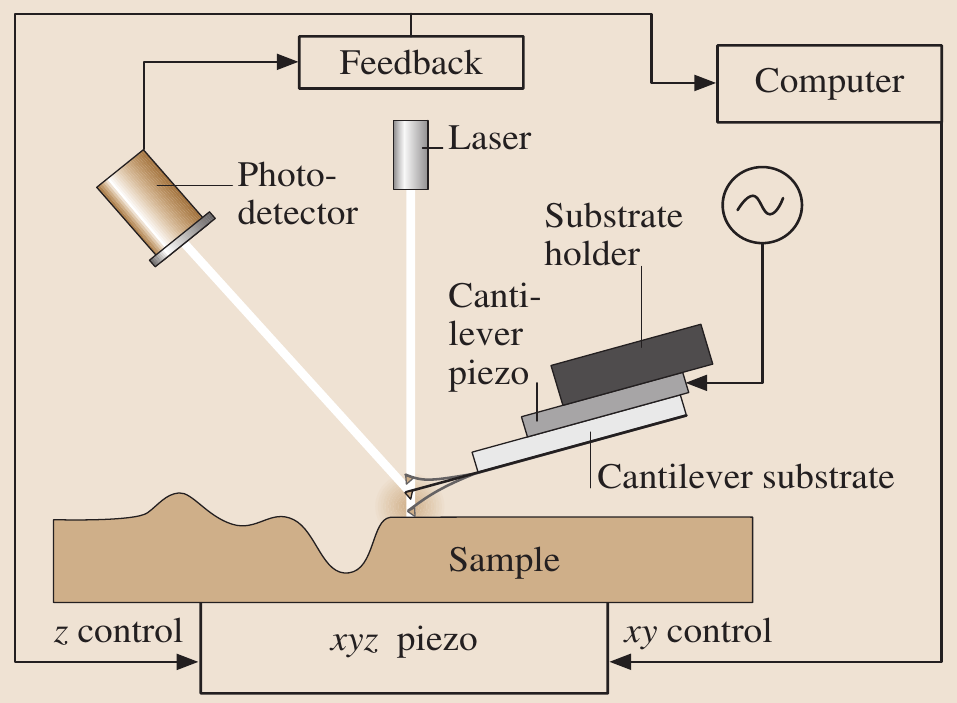
\includegraphics[width=0.5\textwidth]{Tapping_mode}
\caption{Schematic of tapping mode using a feedback mechanism to keep resonant frequency $\omega_0$ of the cantilever constant \cite{Bhushan}.}
\label{fig:Deflection_measurement}
\end{figure}

Similarly to the static mode, we can directly measure the force gradient or use this as a signal for a feedback mechanism that acts on the distance $r$ to keep constant the resonant frequency. An schematic draw is shown in Figure \ref{fig:Deflection_measurement}.

\subsection{Feedback mechanism}
We have mentioned in the previous section that the AFM can be used with or without a feedback mechanism, but since in the experiment we used it both for static and tapping modes, we will describe this technique very briefly.

Feedback mechanisms and feedback parameters are ubiquitous in our life \cite{nanosurf}. For example, when we use a thermostat, the temperature is the feedback parameter, which is set to a a desired one (\emph{setpoint}) and as the temperature in the room changes, it is compared with the temperature setpoint so that a feedback mechanism (e.g. an air conditioner) can act to keep the temperature at the desired value. Mathematically, all these mechanisms are applications of the control theory developed during the 19th century.

\begin{figure}[hbt]
\centering
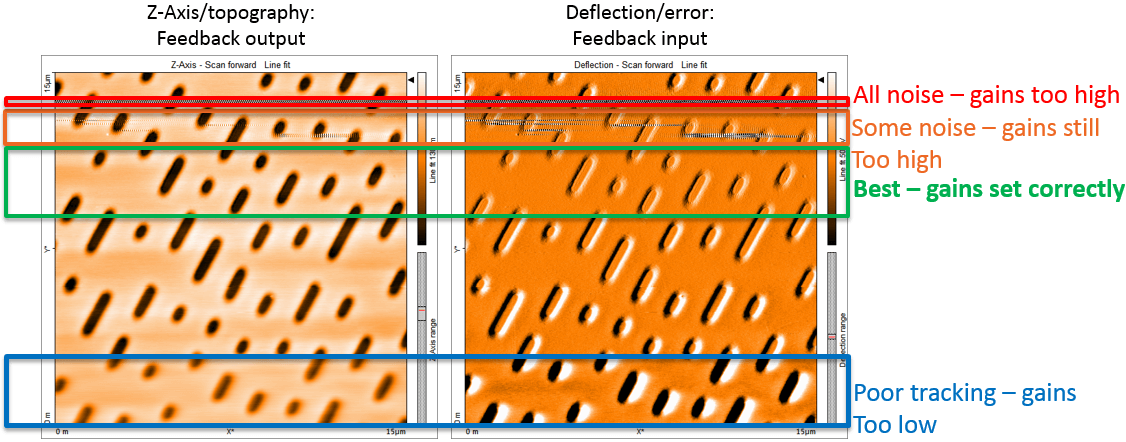
\includegraphics[width=0.8\textwidth]{afm-modes-feedback}
\caption{Feedback input and output signals for different values of PID gains \cite{nanosurf}.}
\label{fig:feedback}
\end{figure}

In our AFM experiment, the feedback parameter that serves as the setpoint in contact mode is the the cantilever deflection. In the tapping mode, it is the cantilever oscillation amplitude. The NaioAFM continuously tries to keep this feedback parameter constant at its setpoint by adjusting the z-piezo to move the cantilever probe up and down. And the resulting z-piezo movements provide the hegight information to create the surface topography.

The feedback loop is controlled through the proportion-integral-derivative control, also referred as the PID gains. These different gains refer to differences in how the feedback loop adjusts to deviations from the setpoint value, i.e. the error signal. In this experiment, the integral gain is the most important one and can have a dramatic effect on the image quality. The proportional gain might provide slight improvement only after the integral gain has been optimized. And the derivative gain is mainly for samples with tall edges.

If gains are set too low, the PID loop is not able to keep the setpoint accurately. Contrary, if gains are chosen too high, the result will be electrical noise in the image interference from the feedback (see Figure \ref{fig:feedback}). This is due to the fact that compensation for a deviation from the setpoint is larger than the error itself.

Nevertheless, gains are not the only parameters that affect the feedback mechanism. The scan rate and, of course, the setpoint value are very important, too. If the scan rate is too fast, the PID loop will not have sufficient time to adjust the feedback parameter to its setpoint value and the height calculated from the z-piezo movement will deviate from the true topography at slopes and near edges. Very slow rates do not affect the quality of the obtained topography since they are not an issue for the PID loop, but they lead to long acquisition times.

Optimization of both scan rate and PID gains are necessary in order to optimize the feedback loop.

\subsection{NaioAFM}

The NaioAFM by Nanosurf \cite{NaioAFM} is the AFM used in this experiment. As the successor of the Easyscan 2, the NaioAFM is a compact AFM designed for new and inexperienced AFM users. It has a closed scanner compartment that helps with acoustic and air current isolation, stage positioners to adjust your sample. The different parts of the scan head including the spot for the cantilever are shown in the Figure \ref{fig:naioafm}. The NaioAFM was placed on an isolation platform to avoid vibration disturbances.

\begin{figure}[hbt]
\centering
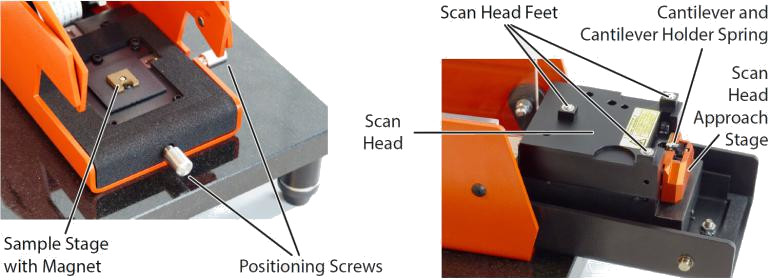
\includegraphics[width=0.9\textwidth]{naioafm2}
\caption{Different parts of the scan head of the NaioAFM instrument \cite{NaioAFM}.}
\label{fig:naioafm}
\end{figure}

\subsection{Gwyddion}

\begin{figure}[ht]
\centering
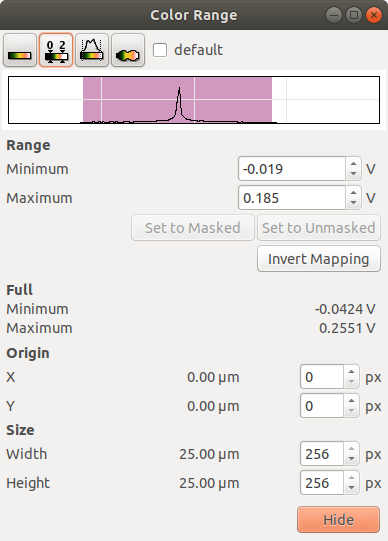
\includegraphics[width=0.4\textwidth]{scale_selection}
\caption{Selection of the highnesses interval}
\label{fig:scale_selection}
\end{figure}

NaioAFM saves the data obtained by the samples in \texttt{.nid} files. These files contain 3-dimensional data of the sample: to every point in the (x,y) plane it is associated a height. The height is shown in 2-dimensional pictures {\color{red}by means of a variable the gray scale}. The lighter the gray is, the higher the z point is.

Thanks to the Gwyddion software, it is possible to partially correct the noisy parts of the pictures manually or by means of some automatic tools. Moreover, the software allow us to model the colour scale by selecting the height range (Figure~\ref{fig:scale_selection}).

Finally, Gwyddion allows us to improve the aesthetics of the images, making them more intuitive. First of all, we can select the colour scale which labels the height of the picture. Secondly, the software is able to generate a 3-dimensional pictures of the sample, as we will see in the following section.

\subsection{AFM artifacts}
When using an AFM, as well as in many other experiments, we may find features which appear in the obtained images that are not present in the observed sample. These are called artifacts \cite{artifacts} and there are four primary sources of artifacts in images measured with AFMs: probes, scanners, image processing and vibrations.

Images measured with an AFM are always a convolution of the probe geometry and the shape of the features being imaged. In order to avoid probe-generated artifacts, the tip should be much smaller than the features being measured. When this condition is not satisfied or if the tip is damaged, features on the sample may appear larger, smaller or with strangely shaped patterns as shown in Figure \ref{fig:artifacts_probe}.

\begin{figure}[H]
\centering
\begin{subfigure}[b]{0.45\textwidth}
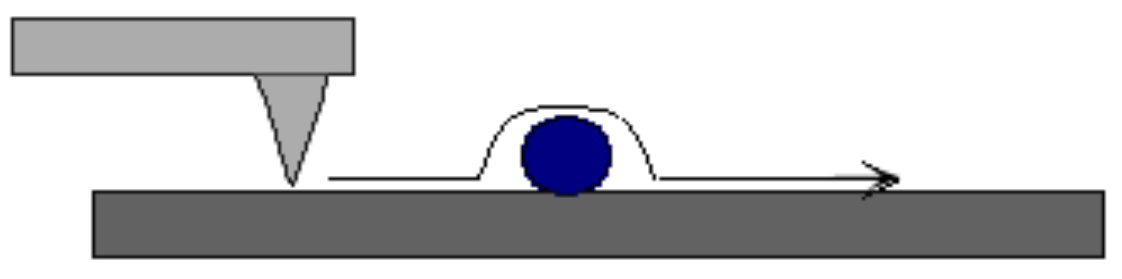
\includegraphics[width=\textwidth]{artifacts_probe_1}
\caption{Feature appears too large}
\label{fig:artifacts_probe_1}
\end{subfigure}
\begin{subfigure}[b]{0.45\textwidth}
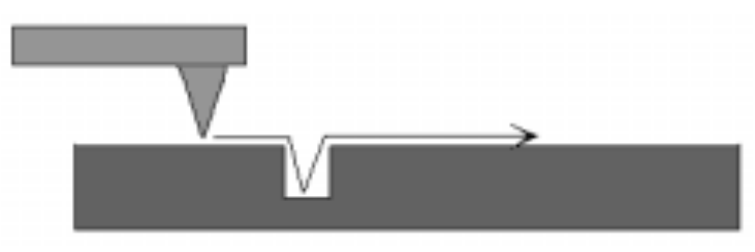
\includegraphics[width=\textwidth]{artifacts_probe_2}
\caption{Feature appears too small}
\label{fig:artifacts_probe_2}
\end{subfigure}\\\vspace{.2cm}
\begin{subfigure}[b]{0.45\textwidth}
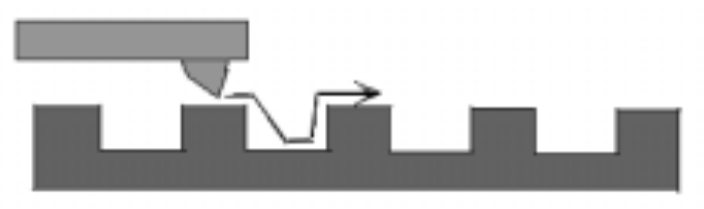
\includegraphics[width=\textwidth]{artifacts_probe_3}
\caption{Distorsion caused by a chipped tip}
\label{fig:artifacts_probe_3}
\end{subfigure}
\caption{Some examples of probe-generated artifacts \cite{artifacts}.}
\label{fig:artifacts_probe}
\end{figure}

Artifacts may also arise due to the motion of the scanner in the X, Y and Z directions. Piezoelectric materials move in a nonlinear motion when a linear voltage ramp is applied. If they are not well calibrated, sizes and forms my appear severely distorted (see Figure \ref{fig:artifacts_scanner_1}). Besides, the geometry of the scanner and the positioning of it relative to the sample can also create artifacts (see Figure \ref{fig:artifacts_scanner_2}).

\begin{figure}[H]
\centering
\begin{subfigure}[b]{0.45\textwidth}
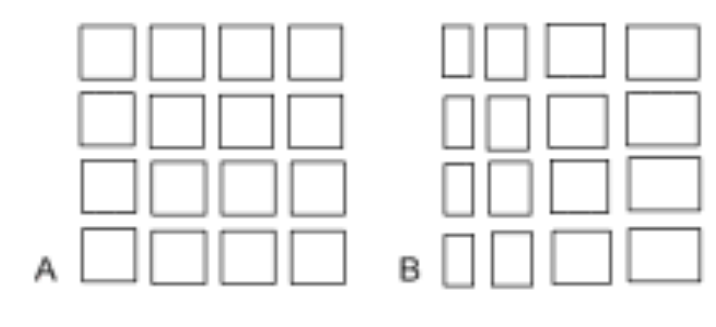
\includegraphics[width=\textwidth]{artifacts_scanner_1}
\caption{A test pattern with squares (left) distorted in the AFM (right) due to nonlinearity of the piezo materials}
\label{fig:artifacts_scanner_1}
\end{subfigure}
\begin{subfigure}[b]{0.45\textwidth}
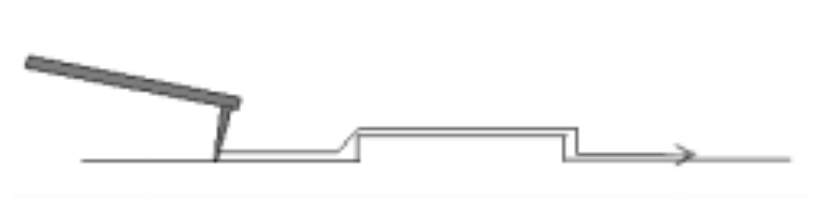
\includegraphics[width=\textwidth]{artifacts_scanner_2}
\caption{Artifact due to the probe sample angle}
\label{fig:artifacts_scanner_2}
\end{subfigure}\\\vspace{.2cm}
\begin{subfigure}[b]{0.45\textwidth}
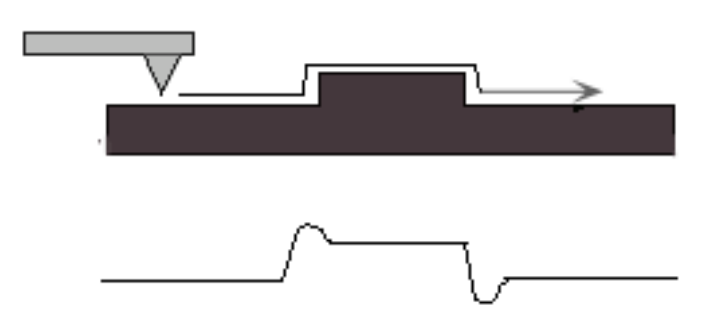
\includegraphics[width=\textwidth]{artifacts_scanner_3}
\caption{Artifact due to overshoot at the leading and trailing edge}
\label{fig:artifacts_scanner_3}
\end{subfigure}
\caption{Some examples of scanner-generated artifacts \cite{artifacts}.}
\label{fig:artifacts_scanner}
\end{figure}

Processing images is a must when dealing with AFM, but additional artifacts can be introduced if the processing software is not properly used. For example, bands that do not correspond to a real structure may appear when subtracting the background (see Figure \ref{fig:artifacts_processing}).

\begin{figure}[H]
\centering
\begin{subfigure}[b]{0.3\textwidth}
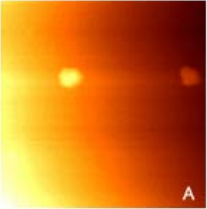
\includegraphics[width=\textwidth]{artifacts_processing_1}
\caption{Image obtained from AFM before any processing}
\label{fig:artifacts_processing_1}
\end{subfigure}
\begin{subfigure}[b]{0.3\textwidth}
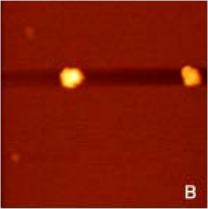
\includegraphics[width=\textwidth]{artifacts_processing_2}
\caption{After a line-by-line leveling with a background correction}
\label{fig:artifacts_processing_2}
\end{subfigure}
\begin{subfigure}[b]{0.3\textwidth}
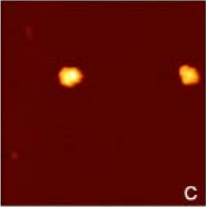
\includegraphics[width=\textwidth]{artifacts_processing_3}
\caption{Particles excluded from the background subtraction}
\label{fig:artifacts_processing_3}
\end{subfigure}\\\vspace{.2cm}
\begin{subfigure}[b]{0.6\textwidth}
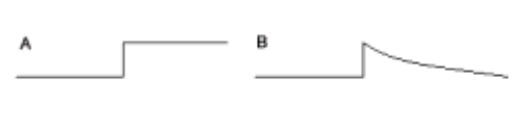
\includegraphics[width=\textwidth]{artifacts_processing_4}
\caption{Artifact due to overshoot at the leading and trailing edge}
\label{fig:artifacts_processing_4}
\end{subfigure}
\caption{Some examples of processing-generated artifacts \cite{artifacts}.}
\label{fig:artifacts_processing}
\end{figure}

Vibrations caused by sound waves can also cause artifacts. Even though the NaioAFM has an isolated compartment do avoid that, even noise derived from a person talking in the same room as the AFM can be observed (see Figure \ref{fig:artifacts_vibrations}). Additionally, surface contamination on the sample (see Figure \ref{fig:artifacts_contamination})or electronic noise (see Figure \ref{fig:artifacts_electronics}) among others can also cause artefacts.

\begin{figure}[H]
\centering
\begin{subfigure}[b]{0.45\textwidth}
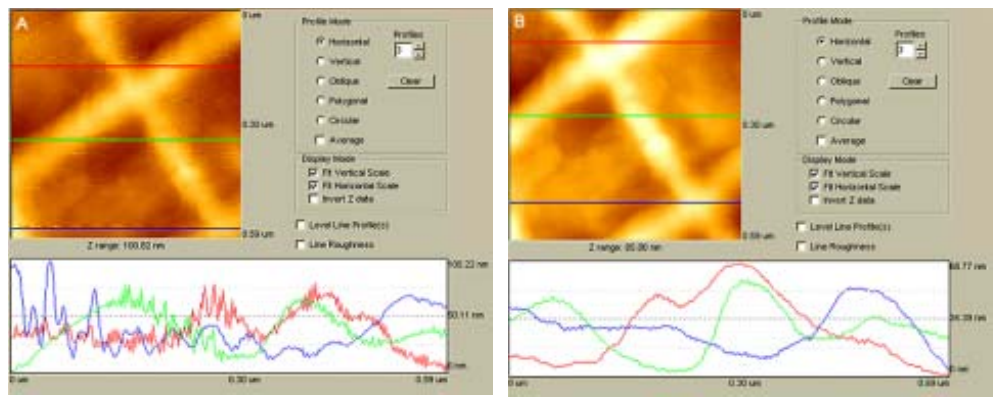
\includegraphics[width=\textwidth]{artifacts_vibrations}
\caption{Without noise (left) and with noise (right)}
\label{fig:artifacts_vibrations}
\end{subfigure}
\begin{subfigure}[b]{0.45\textwidth}
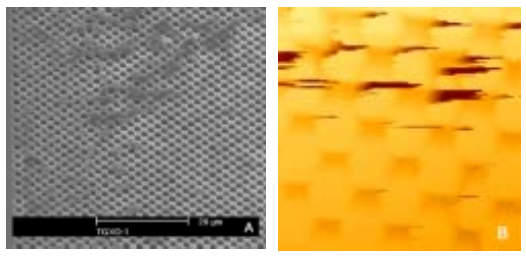
\includegraphics[width=\textwidth]{artifacts_contamination}
\caption{Sample contamination shown in a SEM image (left) and in an AFM one (right)}
\label{fig:artifacts_contamination}
\end{subfigure}\\\vspace{.2cm}
\begin{subfigure}[b]{0.45\textwidth}
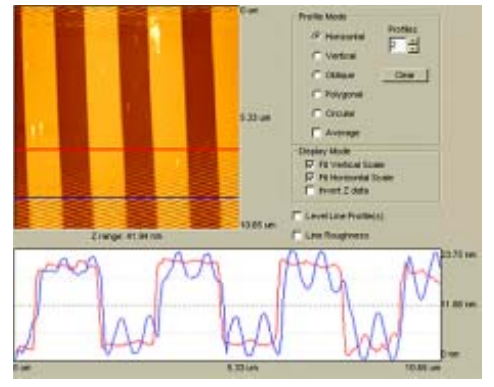
\includegraphics[width=\textwidth]{artifacts_electronics}
\caption{Electronic noise}
\label{fig:artifacts_electronics}
\end{subfigure}
\caption{Some examples of artifacts caused by sound noise, contamination and electronic noise \cite{artifacts}.}
\label{fig:artifacts_others}
\end{figure}

\section{Results and discussion}
In this section we will describe the analysis of the 3 different samples using both static and tapping mode.

\subsection{Static mode}
\subsubsection{Calibration}
First, we used a \emph{calibration sample} with a known surface in order to test the tip and the software used to obtain our data. This sample was the Calibration Standard \texttt{HS-100MG} and it had 6 different surfaces (see Figure \ref{fig:HS-100MG}).

\begin{figure}[H]
\centering
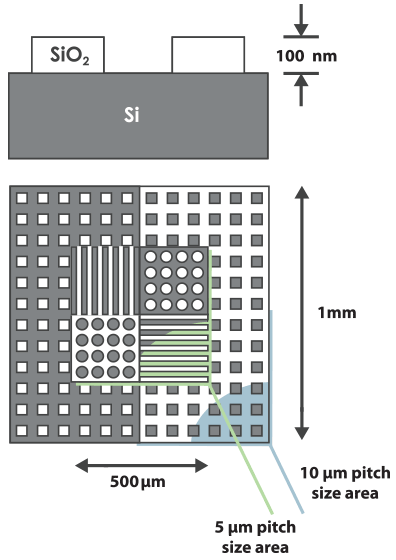
\includegraphics[width=0.3\textwidth]{HS-100MG}
\caption{Dimensions of the calibration sample HS-100MG.}
\label{fig:HS-100MG}
\end{figure}

We fixed the sample in the centre of the AFM and used the camera installed inside our Nanosurf NaioAFM equipment to place the tip in the different surfaces (shown in Figure~\ref{fig:cal_sam}).

\begin{figure}[ht]
\centering
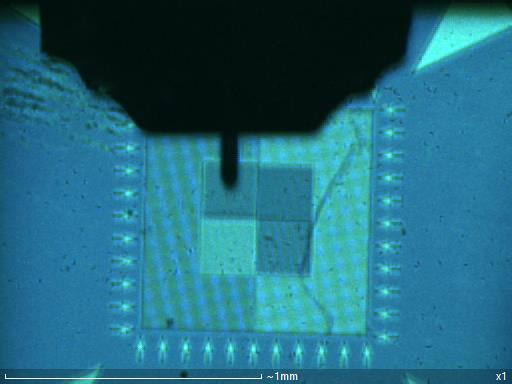
\includegraphics[scale=0.4]{calibration_sample.JPG}
\caption{Calibration sample view from the camera installed in Nanosurf NaioAFM}
\label{fig:cal_sam}
\end{figure}

Once we had chosen the surface which we wanted to analyse, we put the tip as close as possible to the sample without making them contact by using the software. Then, using the \emph{approach mode}, we brought the tip in contact with the surface. This mode uses the setpoint and the feedback mechanism to very slowly put the tip in contact minimizing the risk of breaking the tip.

In the following pictures, it is possible to see 3 different shapes captured from our calibration sample:

\begin{figure}[H]
\centering
\begin{subfigure}[b]{0.45\textwidth}
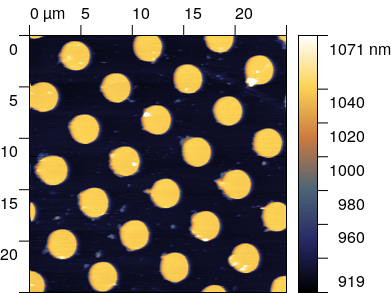
\includegraphics[width=\textwidth]{sm_points}
\caption{Points surface}
\label{fig:sm_points}
\end{subfigure}
\begin{subfigure}[b]{0.45\textwidth}
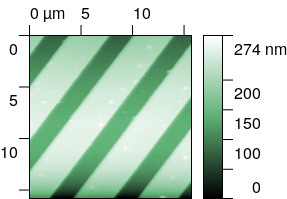
\includegraphics[width=\textwidth]{sm_raws}
\caption{Raws surface}
\label{fig:sm_raws}
\end{subfigure}\\\vspace{.2cm}
\begin{subfigure}[b]{0.45\textwidth}
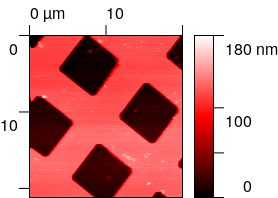
\includegraphics[width=\textwidth]{sm_squares}
\caption{Squares surface}
\label{fig:sm_squares}
\end{subfigure}
\begin{subfigure}[b]{0.45\textwidth}
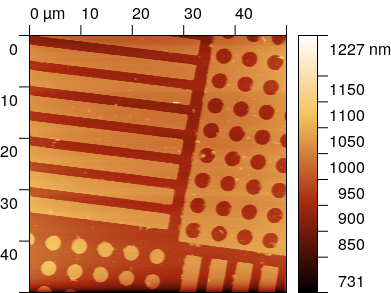
\includegraphics[width=\textwidth]{sm_border}
\caption{Border between more surfaces}
\label{fig:sm_border}
\end{subfigure}
\caption{Some pictures of the calibration sample}
\end{figure}

The previous pictures have been processed using Gwyddion software. First of all we used some masks to eliminate automatically some imperfections, as for instance orizontal tears caused by abrupt movements of the tip. Secondly, we adjusted the high scale in which the shade of colors had to variate. Finally, we chosed 4 different colour scales in order to better distinguish the 4 pictures.

We can notice that the pictures showing the 3 surfaces are $\SI{25}{\micro m} \times \SI{25}{\micro m}$, while the last picture has a larger area $\SI{50}{\micro m} \times \SI{50}{\micro m}$ in order to let us see part of the all 4 surfaces. We can also observe that the range of the z-axis has been chosen a bit larger in the last picture ($\Delta V=189V+27V=216V$) {\color{red}because we are describing more surfaces in only one image.} Finally we report the 3D image got from the data taken in the border:

\begin{figure}[ht]
\centering
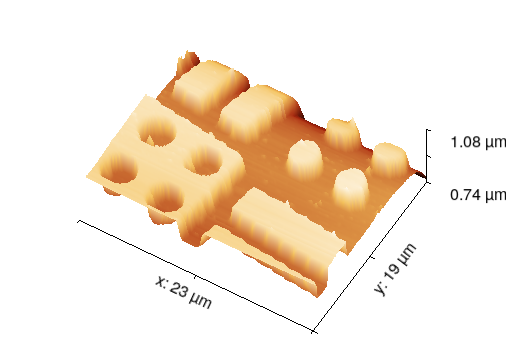
\includegraphics[scale=0.47]{sm_border_3D}
\caption{3D plot of the calibration sample's border}
\label{fig: cal sam border}
\end{figure}

\subsubsection{Sample 1}
The first sample was {\color{Red} I don't remember the materials}. We took the measurements moving the tip in 2 different directions that were oriented by $\pi /4$ between them. We can observe this fact in the following pictures:

\begin{figure}[H]
\centering
\begin{subfigure}[b]{0.45\textwidth}
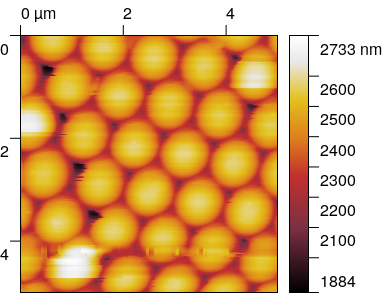
\includegraphics[width=\textwidth]{sm_sample1}
\caption{Sample 1: first direction}
\label{fig:}
\end{subfigure}
\begin{subfigure}[b]{0.45\textwidth}
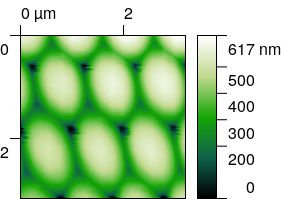
\includegraphics[width=\textwidth]{sm_sample1_dir2}
\caption{Sample 1: second direction}
\label{fig:}
\end{subfigure}\\\vspace{.2cm}
\begin{subfigure}[b]{0.45\textwidth}
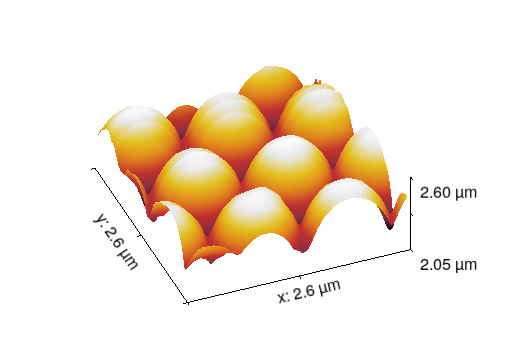
\includegraphics[width=\textwidth]{sm_sample1_3D}
\caption{Sample 1: first direction, 3D plot}
\label{fig:}
\end{subfigure}
\begin{subfigure}[b]{0.45\textwidth}
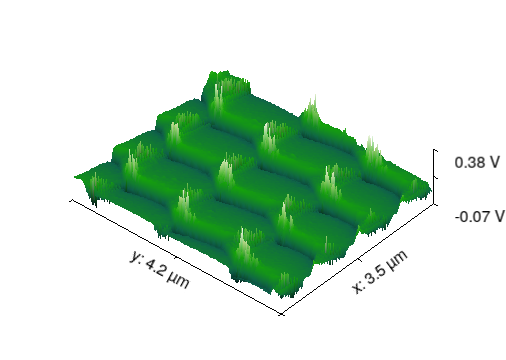
\includegraphics[width=\textwidth]{sm_sample1_dir2_3D}
\caption{Sample 1: second direction, 3D plot}
\label{fig:}
\end{subfigure}
\caption{Sample 1}
\end{figure}

We can see from the pictures that the 2 directions give us a exagonal beehive plot. The second direction makes the exagons more stratched.%, but the highness is approximatively the same ($\Delta V_{dir1} \simeq \Delta V_{dir2}$).

\subsubsection{Sample 2}
The second sample is BOH. We can see from Figure~\ref{fig:sample2_set} that the surface of this material was scratched and full of imperfections.

\begin{figure}[ht]
\centering
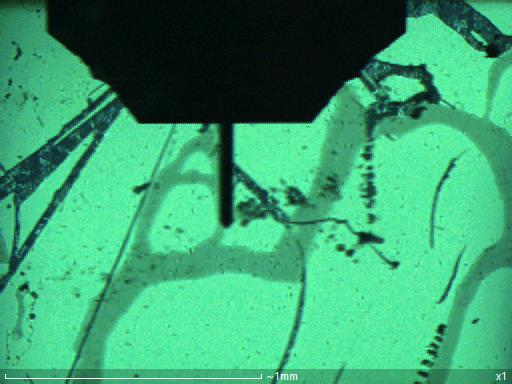
\includegraphics[scale=0.4]{sm_sample2_set.JPG}
\caption{Picture of sample 2 from the camera installed in Nanosurf NaioAFM}
\label{fig:sample2_set}
\end{figure}

We have have notice that the only part of the material which has a plot is the light green part (Figure~\ref{fig:sample2_set}). Therefore we have decided to take measurments inside the plot and in the border (the position of the tip is shown in Figure~\ref{fig:sample2_set}).

\begin{figure}[H]
\centering
\begin{subfigure}[b]{0.45\textwidth}
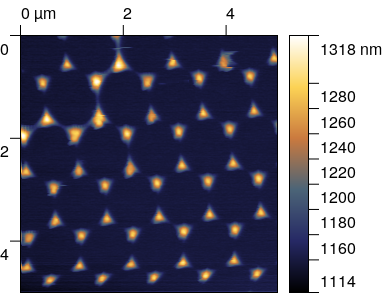
\includegraphics[width=\textwidth]{sm_sample2}
\caption{Sample 2: inside the plot}
\label{fig:}
\end{subfigure}
\begin{subfigure}[b]{0.45\textwidth}
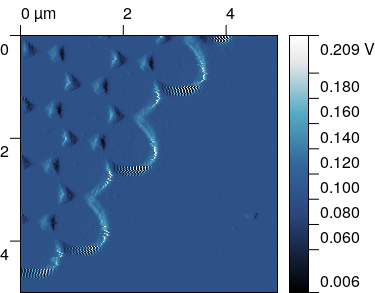
\includegraphics[width=\textwidth]{sm_sample2_border}
\caption{Sample 2: border}
\label{fig:}
\end{subfigure}\\\vspace{.2cm}
\begin{subfigure}[b]{0.45\textwidth}
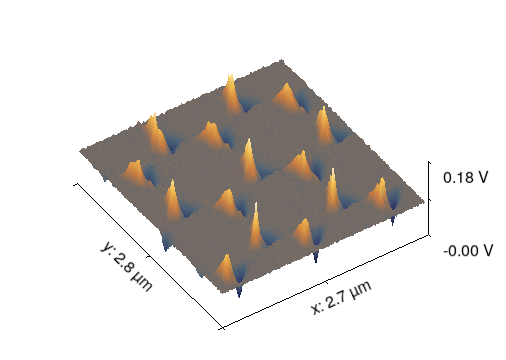
\includegraphics[width=\textwidth]{sm_sample2_3D}
\caption{Sample 2: inside the plot, 3D plot}
\label{fig:}
\end{subfigure}
\begin{subfigure}[b]{0.45\textwidth}
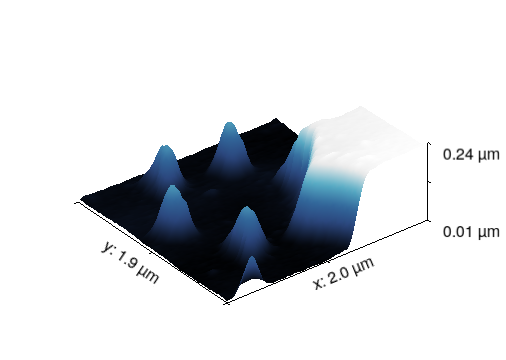
\includegraphics[width=\textwidth]{sm_sample2_border_3D}
\caption{Sample 1: border, 3D plot}
\label{fig:}
\end{subfigure}
\caption{Sample 2}
\end{figure}

We can observe that the plot reminds a set of stars. Moreover, we can see that the surface outside this plot is flat compared to the edges of the star.

\subsubsection{Sample 3}
As we can notice from the following picture (Figure~\ref{fig:sample3_set}), even the third sample was characterized by scratches and imperfections.

\begin{figure}[ht]
\centering
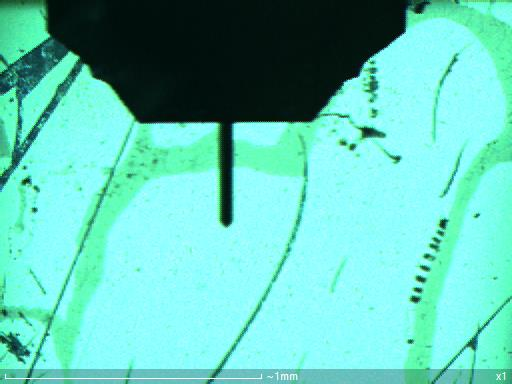
\includegraphics[scale=0.4]{sm_sample3_set}
\caption{Picture of sample 3 from the camera installed in Nanosurf NaioAFM}
\label{fig:sample3_set}
\end{figure}

This time we took only one measurement in the center of the light green part as shown below:

\begin{figure}[H]
\centering
\begin{subfigure}[b]{0.45\textwidth}
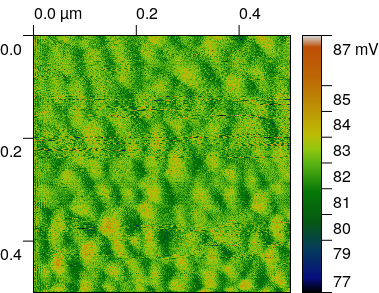
\includegraphics[width=\textwidth]{sm_sample3}
\caption{Sample 3: inside the plot}
\label{fig:}
\end{subfigure}
\begin{subfigure}[b]{0.45\textwidth}
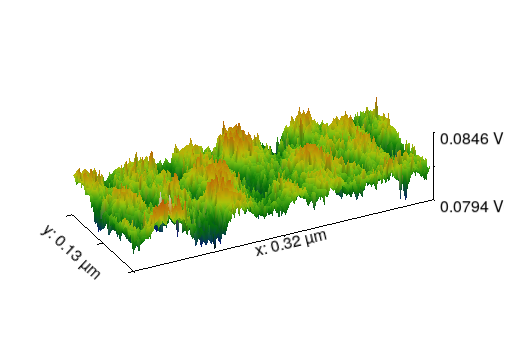
\includegraphics[width=\textwidth]{sm_sample3_3D_improved}
\caption{Sample 3: 3D plot}
\label{fig:}
\end{subfigure}
\caption{Sample 3}
\end{figure}

In this last sample we can notice a hilly surface. In order to observe this plot, the precision in the highness had to be improved, indeed we can see that the $V$ scale is of the order of $mV$ instead of $V$ as before.

\subsection{Tapping mode}
\subsubsection{Calibration}
Even in this case, the first stap was the measurement of the calibration sample.

\begin{figure}[H]
\centering
\begin{subfigure}[b]{0.45\textwidth}
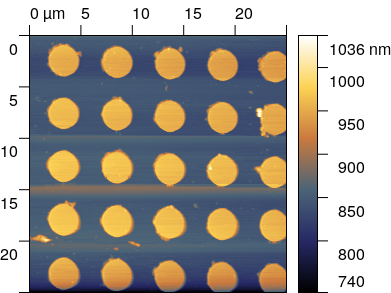
\includegraphics[width=\textwidth]{tm_points}
\caption{Points surface}
\label{fig:}
\end{subfigure}
\begin{subfigure}[b]{0.45\textwidth}
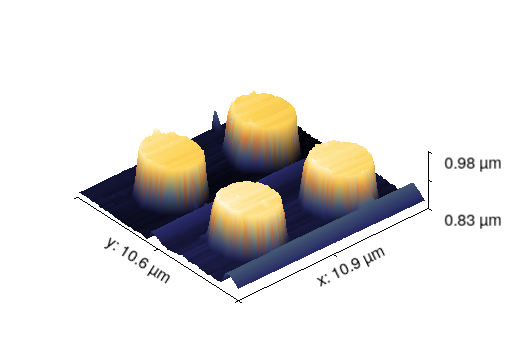
\includegraphics[width=\textwidth]{tm_points_3D}
\caption{Points surface, 3D plot}
\label{fig:sm_raws}
\end{subfigure}\\\vspace{.2cm}
\begin{subfigure}[b]{0.45\textwidth}
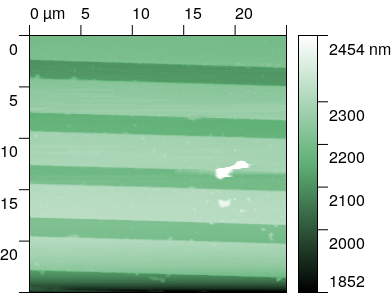
\includegraphics[width=\textwidth]{tm_raws}
\caption{Raws surface}
\label{fig:}
\end{subfigure}
\begin{subfigure}[b]{0.45\textwidth}
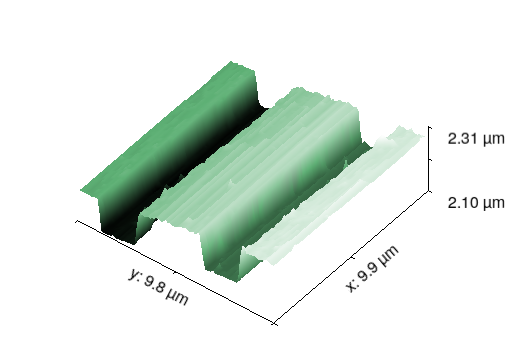
\includegraphics[width=\textwidth]{tm_raws_3D}
\caption{Raws surface, 3D plot}
\label{fig:}
\end{subfigure}\\\vspace{.2cm}
\begin{subfigure}[b]{0.45\textwidth}
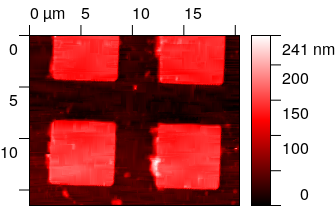
\includegraphics[width=\textwidth]{tm_squares}
\caption{Squares surface}
\label{fig:}
\end{subfigure}
\begin{subfigure}[b]{0.45\textwidth}
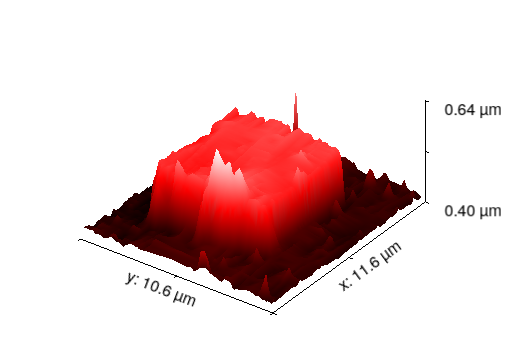
\includegraphics[width=\textwidth]{tm_squares_3D}
\caption{Squares surface, 3D plot}
\label{fig:sm_border}
\end{subfigure}
\caption{Some pictures of the calibration sample}
\end{figure}

Looking at the 3 dimensional plots, we can see that in this case the measurements are far more precise. In fact observing the border between two different highnesses, we notice that in the static mode we had large peaks (Figure~\ref{fig: cal sam border}), while in the tapping mode the border is far more clean.

\subsubsection{Sample 1}

\begin{figure}[H]
\centering
\begin{subfigure}[b]{0.45\textwidth}
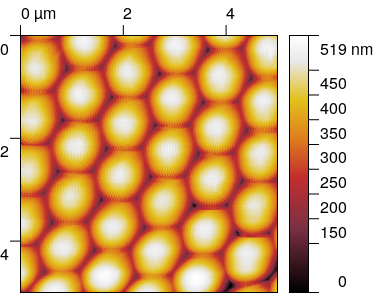
\includegraphics[width=\textwidth]{tm_sample1}
\caption{Sample 1 in tapping mode}
\label{fig:}
\end{subfigure}
\begin{subfigure}[b]{0.45\textwidth}
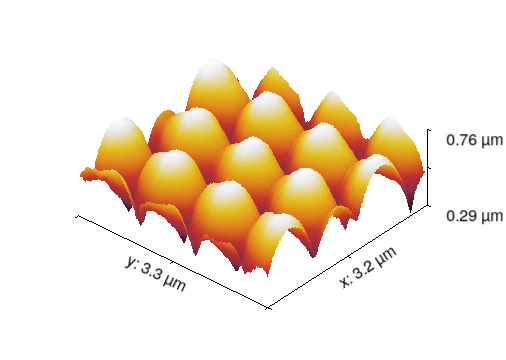
\includegraphics[width=\textwidth]{tm_sample1_3D}
\caption{Sample 1 in tapping mode, 3D plot}
\label{fig:}
\end{subfigure}
\end{figure}
\subsubsection{Sample 2}
\begin{figure}[H]
\centering
\begin{subfigure}[b]{0.45\textwidth}
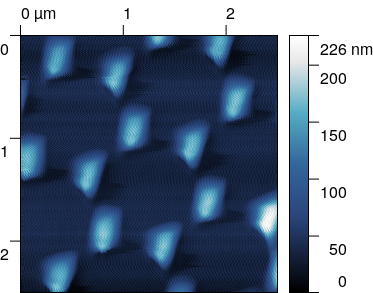
\includegraphics[width=\textwidth]{tm_sample2}
\caption{Sample 2 in tapping mode}
\label{fig:}
\end{subfigure}
\begin{subfigure}[b]{0.45\textwidth}
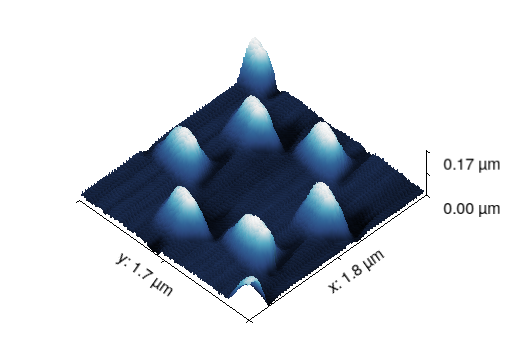
\includegraphics[width=\textwidth]{tm_sample2_3D}
\caption{Sample 2 in tapping mode, 3D plot}
\label{fig:}
\end{subfigure}
\end{figure}

\subsubsection{Sample 3}

\begin{figure}[H]
\centering
\begin{subfigure}[b]{0.45\textwidth}
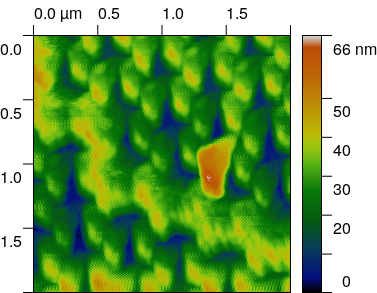
\includegraphics[width=\textwidth]{tm_sample3}
\caption{Sample 3 in tapping mode}
\label{fig:}
\end{subfigure}
\begin{subfigure}[b]{0.45\textwidth}
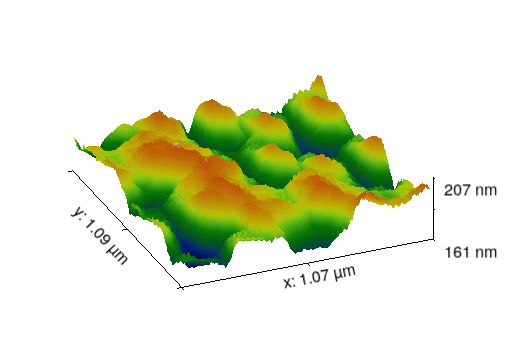
\includegraphics[width=\textwidth]{tm_sample3_3D}
\caption{Sample 3 in tapping mode, 3D plot}
\label{fig:}
\end{subfigure}
\end{figure}

\section{Conclusions}


\nocite{*}
\newpage
\bibliographystyle{unsrt}
\bibliography{references}
\end{document}